\documentclass{article}
\usepackage{amsfonts} 
\usepackage{amsmath}
\usepackage{hyperref}
\usepackage{graphicx}
\usepackage{subcaption}
\usepackage{booktabs}
\usepackage{makecell}
\usepackage{multirow}
%\usepackage{placeins}

\begin{document}


\section{Model}
\par The $d$ dimensional torus $\mathbb{T}^d$ can be defined as $\left(\mathbb{R}/n\mathbb{Z}\right)^d$ for some natural $n$. And we can represent this as a cell-complex with cubical $d$-dimensional cells $\left(\mathbb{Z}/n\mathbb{Z}\right)^d + [0, 1]^d$ and all their $k$-faces for $k=0, ..., d$.
\par We randomly assume the filtration value for each $k$-face uniformly distributed in $[k, k+1]$. This filtration on segmented torus will corespond some real filtration $f: mathbb{T}^d\to\mathbb{R}$, s.t. the $d$-dimensional cells will corespond the local maximums, vertices will corespond the local minimums and other $k$-faces will be saddles.
\begin{figure}[h!]
    \centering
    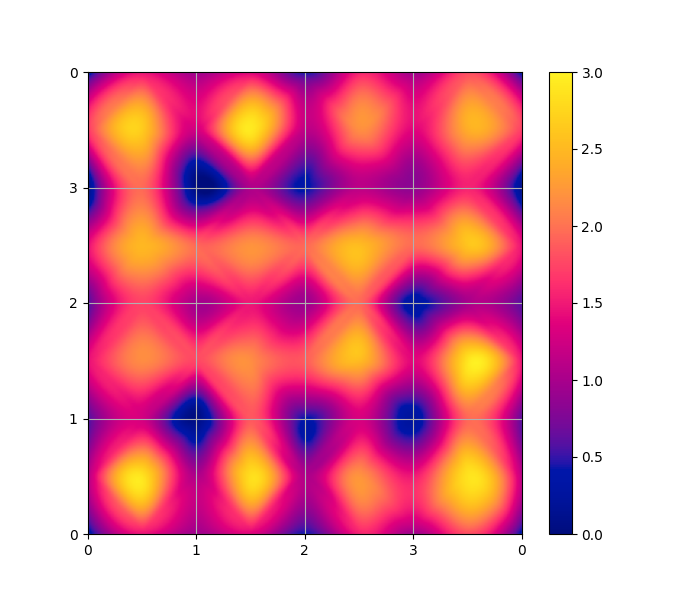
\includegraphics[width=0.6\textwidth]{pics/torus scores/2d-example.png}
    \caption{The example of the filtration $f:\mathbb{T}^2\to\mathbb{R}$, s.t. there are local minimums in the vertices, saddles in the middle of edges, and the local maximums in the centers of square cells.}
    \label{fig:example2d}
\end{figure}
\par Let's call models like this as Barycentric Cubical Torus.
\par The $d$-dimensional torus model will contain $2^d$ essential cycles. So we will add some auxiliary cells to kill them:
The first we will add $-1$-dimensional cell with the filtration value 0 which border will be all vertices. After this the cell which id birth of the first connected component will be paired with new auxiliary cell as the death of empty set. 
And then for each dimendion $k\in\{2, ..., d\}$ we will add $C_d^k$ $k$-dimensional cells, which border will be all $(k-1)$ dimensial cells, satisfyed the $(d - k)$ constraints like $x_i = 0$. These auxiliary cells will be paired with previusly unpaired cells as deaths of essential cycles.

\section{Poset Scores}
\subsection{Scores Description}
\par We have computed the following scores for the objects in the depth poset of the extended barycentric cubical torus:
\begin{itemize}
\item \textbf{cycles\_dimension} - Returns the dimension of space of cycles in reduction.
\item \textbf{height} - Returns the poset height - the length of the longest chain.
\item \textbf{number\_of\_components} - Returns the number of connetcted components in the poset
\item \textbf{number\_of\_maximal\_nodes} - Returns the number of maximal nodes.
\item \textbf{number\_of\_minimal\_nodes} - Returns the number of minimal nodes.
\item \textbf{number\_of\_nodes} - Returns the number of nodes in the poset.
\item \textbf{number\_of\_relations} - Returns the number of relations in the transitive reduction.
\end{itemize}
\subsection{Scores}
\par We can see the score values in the following figures:
\begin{center}
\begin{tabular}{llllll}
\toprule
dim & \multicolumn{3}{r}{2} & 3 & 1 \\
reduction & full & row reduction & column reduction & full & full \\
\midrule
cycles\_dimension & Fig. \ref{fig:cyclesdimension-full2} &  &  & Fig. \ref{fig:cyclesdimension-full3} & Fig. \ref{fig:cyclesdimension-full1} \\
height & Fig. \ref{fig:height-full2} &  &  & Fig. \ref{fig:height-full3} & Fig. \ref{fig:height-full1} \\
number\_of\_components & Fig. \ref{fig:numberofcomponents-full2} & Fig. \ref{fig:numberofcomponents-rowreduction2} & Fig. \ref{fig:numberofcomponents-columnreduction2} &  &  \\
number\_of\_maximal\_nodes & Fig. \ref{fig:numberofmaximalnodes-full2} & Fig. \ref{fig:numberofmaximalnodes-rowreduction2} & Fig. \ref{fig:numberofmaximalnodes-columnreduction2} &  &  \\
number\_of\_minimal\_nodes & Fig. \ref{fig:numberofminimalnodes-full2} & Fig. \ref{fig:numberofminimalnodes-rowreduction2} & Fig. \ref{fig:numberofminimalnodes-columnreduction2} &  &  \\
number\_of\_nodes & Fig. \ref{fig:numberofnodes-full2} &  &  & Fig. \ref{fig:numberofnodes-full3} & Fig. \ref{fig:numberofnodes-full1} \\
number\_of\_relations & Fig. \ref{fig:numberofrelations-full2} &  &  & Fig. \ref{fig:numberofrelations-full3} & Fig. \ref{fig:numberofrelations-full1} \\
\bottomrule
\end{tabular}

\end{center}
    \begin{figure}[h!]
        \centering
        \hspace*{-0.24\textwidth}
        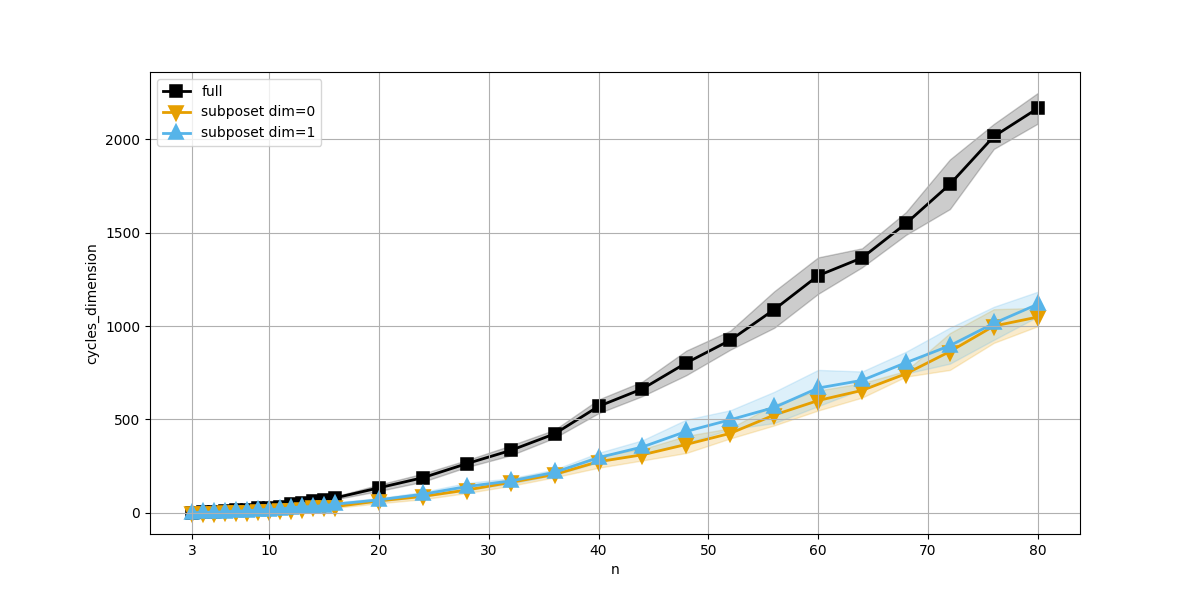
\includegraphics[width=1.4\textwidth]{pics/extended torus scores/score=cycles-dimension, dim=2, object=full.png}
        \caption{Score cycles\_dimension values for the full poset of $\mathbb{T}_n^{2}$.}
        \label{fig:cyclesdimension-full2}
    \end{figure}
    \begin{figure}[h!]
        \centering
        \hspace*{-0.24\textwidth}
        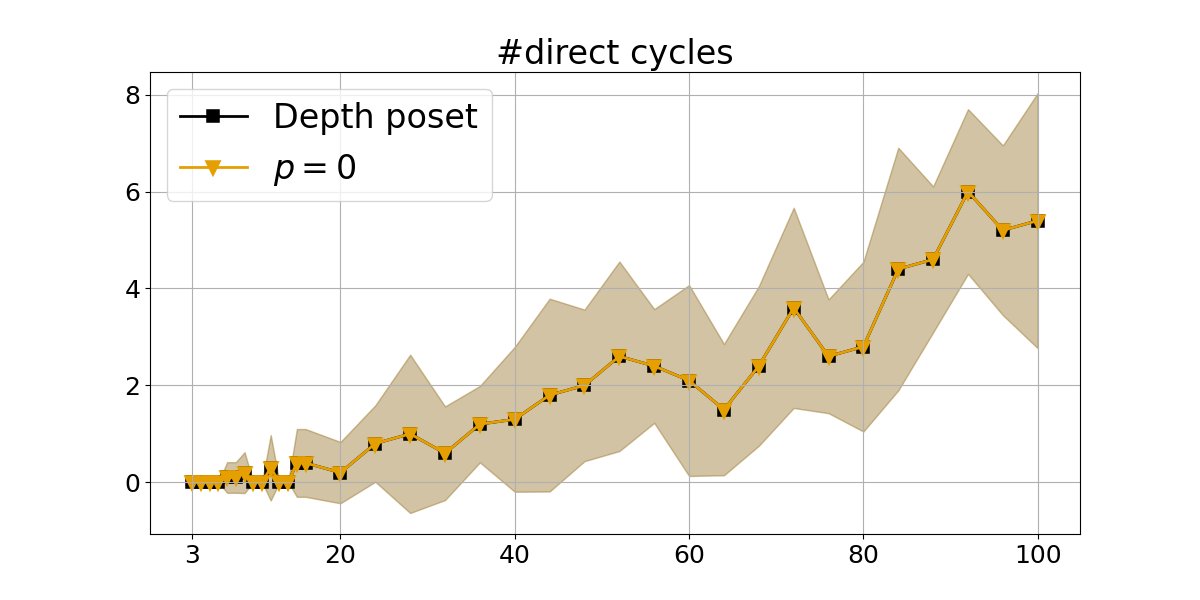
\includegraphics[width=1.4\textwidth]{pics/extended torus scores/score=cycles-dimension, dim=1, object=full.png}
        \caption{Score cycles\_dimension values for the full poset of $\mathbb{T}_n^{1}$.}
        \label{fig:cyclesdimension-full1}
    \end{figure}
    \begin{figure}[h!]
        \centering
        \hspace*{-0.24\textwidth}
        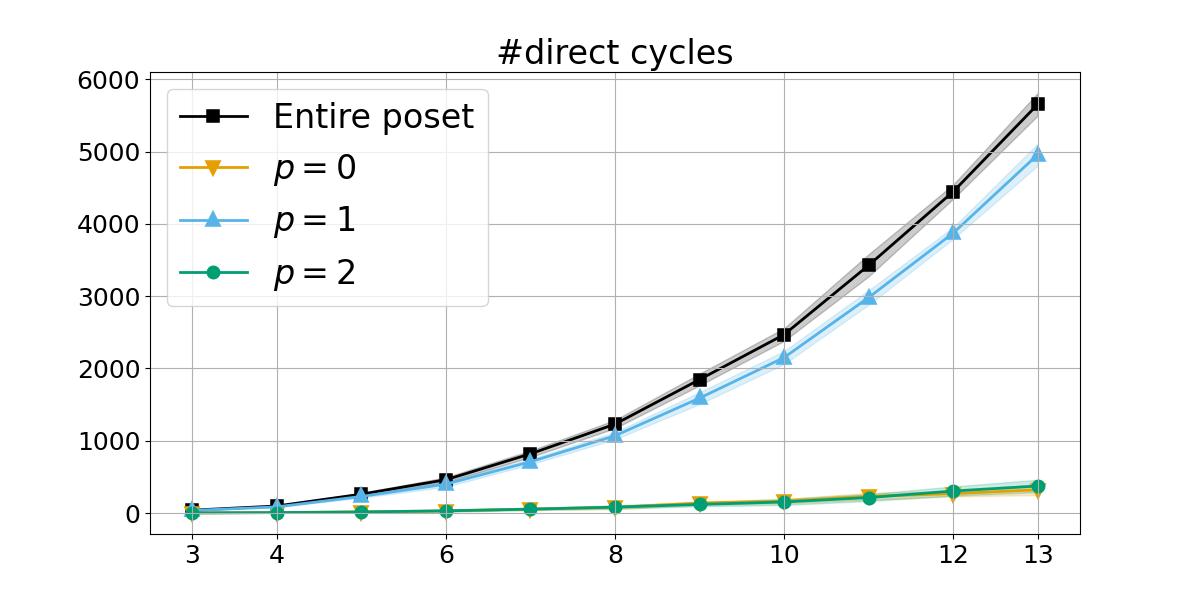
\includegraphics[width=1.4\textwidth]{pics/extended torus scores/score=cycles-dimension, dim=3, object=full.png}
        \caption{Score cycles\_dimension values for the full poset of $\mathbb{T}_n^{3}$.}
        \label{fig:cyclesdimension-full3}
    \end{figure}
    \begin{figure}[h!]
        \centering
        \hspace*{-0.24\textwidth}
        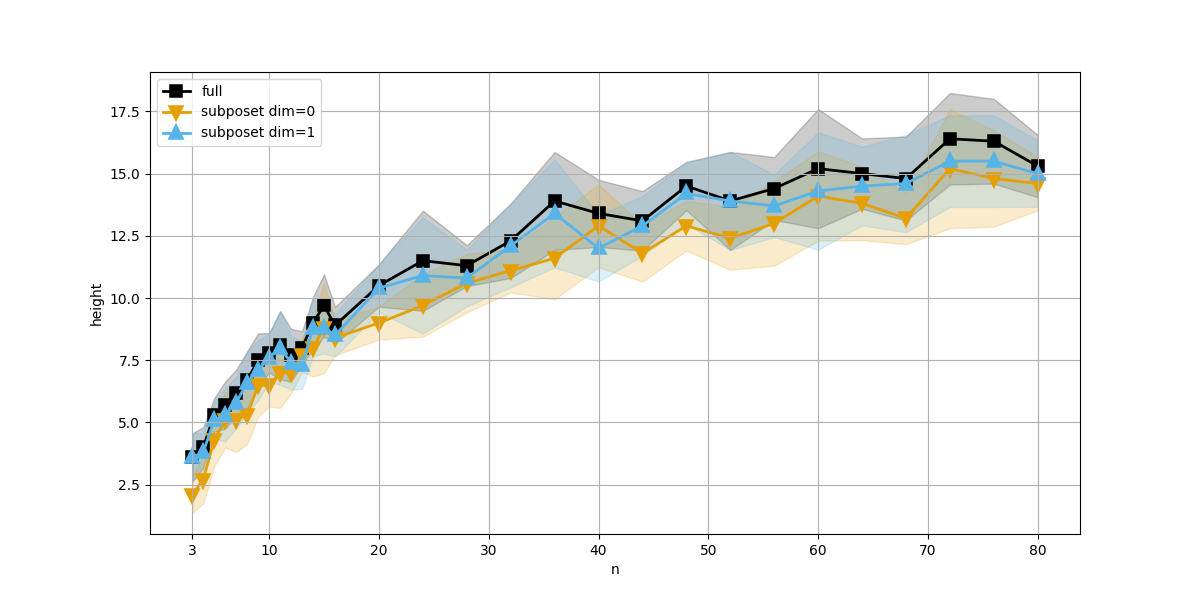
\includegraphics[width=1.4\textwidth]{pics/extended torus scores/score=height, dim=2, object=full.png}
        \caption{Score height values for the full poset of $\mathbb{T}_n^{2}$.}
        \label{fig:height-full2}
    \end{figure}
    \begin{figure}[h!]
        \centering
        \hspace*{-0.24\textwidth}
        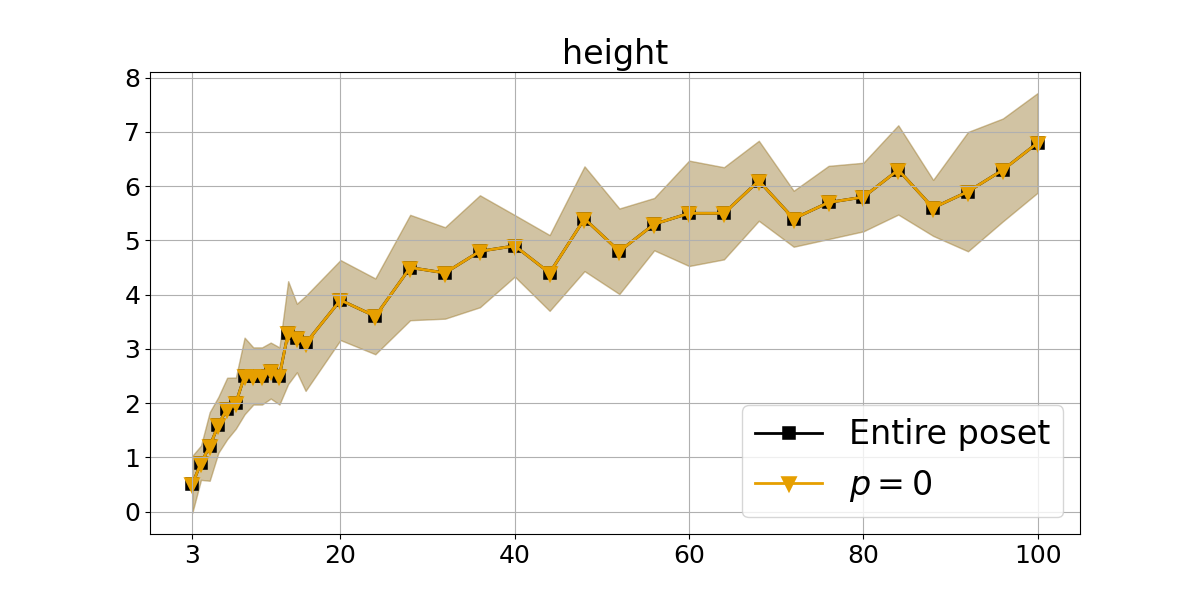
\includegraphics[width=1.4\textwidth]{pics/extended torus scores/score=height, dim=1, object=full.png}
        \caption{Score height values for the full poset of $\mathbb{T}_n^{1}$.}
        \label{fig:height-full1}
    \end{figure}
    \begin{figure}[h!]
        \centering
        \hspace*{-0.24\textwidth}
        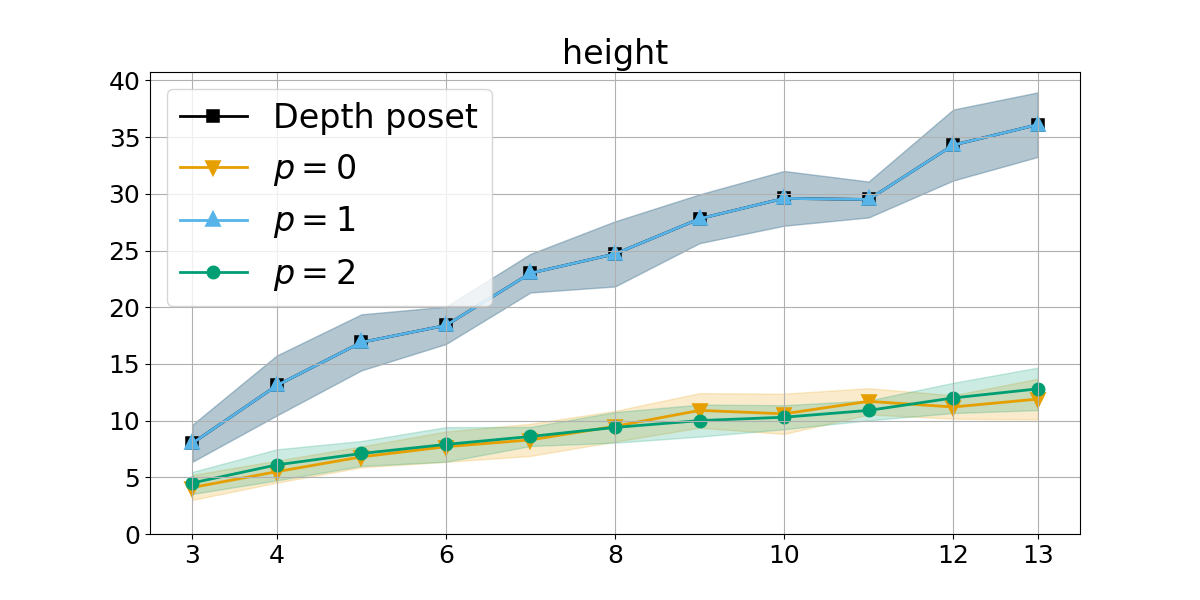
\includegraphics[width=1.4\textwidth]{pics/extended torus scores/score=height, dim=3, object=full.png}
        \caption{Score height values for the full poset of $\mathbb{T}_n^{3}$.}
        \label{fig:height-full3}
    \end{figure}
    \begin{figure}[h!]
        \centering
        \hspace*{-0.24\textwidth}
        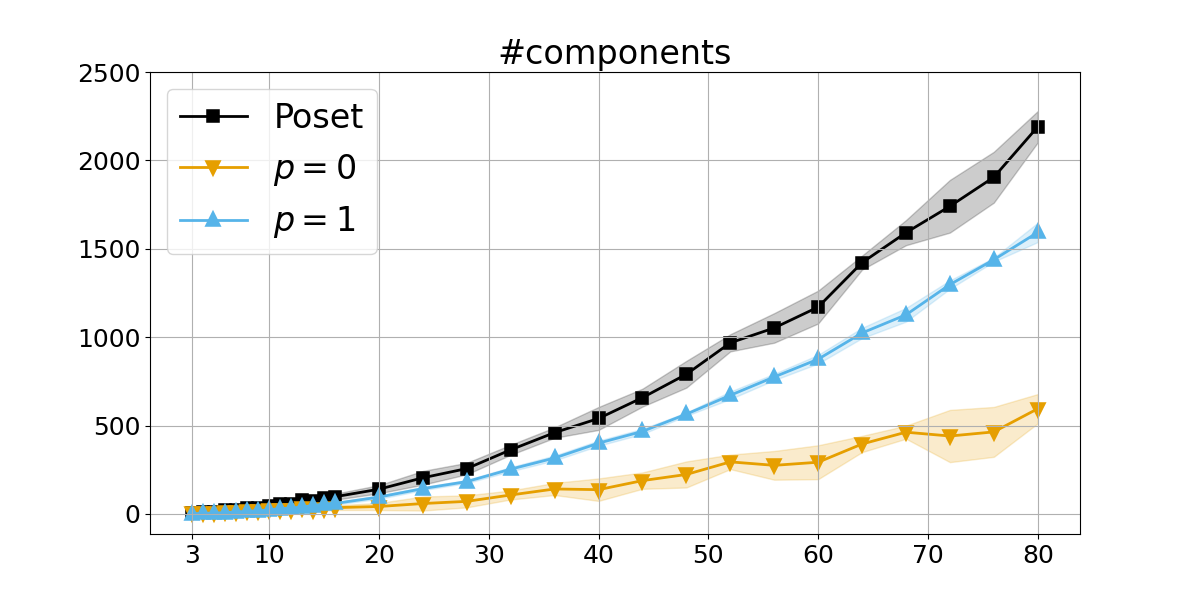
\includegraphics[width=1.4\textwidth]{pics/extended torus scores/score=number-of-components, dim=2, object=row reduction.png}
        \caption{Score number\_of\_components values for the row reduction poset of $\mathbb{T}_n^{2}$.}
        \label{fig:numberofcomponents-rowreduction2}
    \end{figure}
    \begin{figure}[h!]
        \centering
        \hspace*{-0.24\textwidth}
        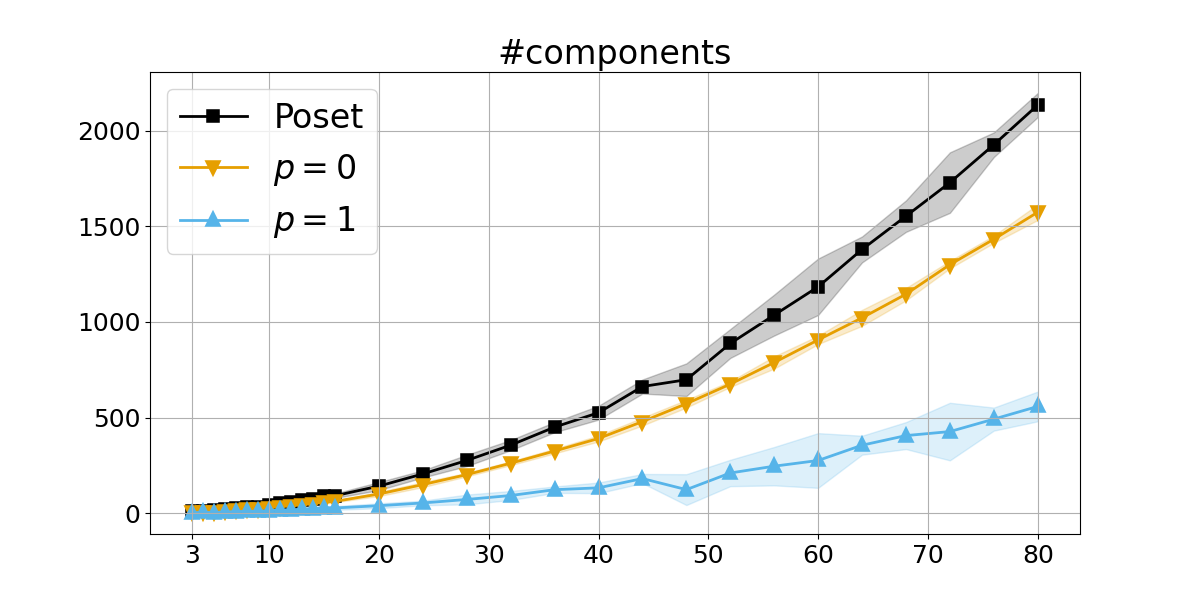
\includegraphics[width=1.4\textwidth]{pics/extended torus scores/score=number-of-components, dim=2, object=column reduction.png}
        \caption{Score number\_of\_components values for the column reduction poset of $\mathbb{T}_n^{2}$.}
        \label{fig:numberofcomponents-columnreduction2}
    \end{figure}
    \begin{figure}[h!]
        \centering
        \hspace*{-0.24\textwidth}
        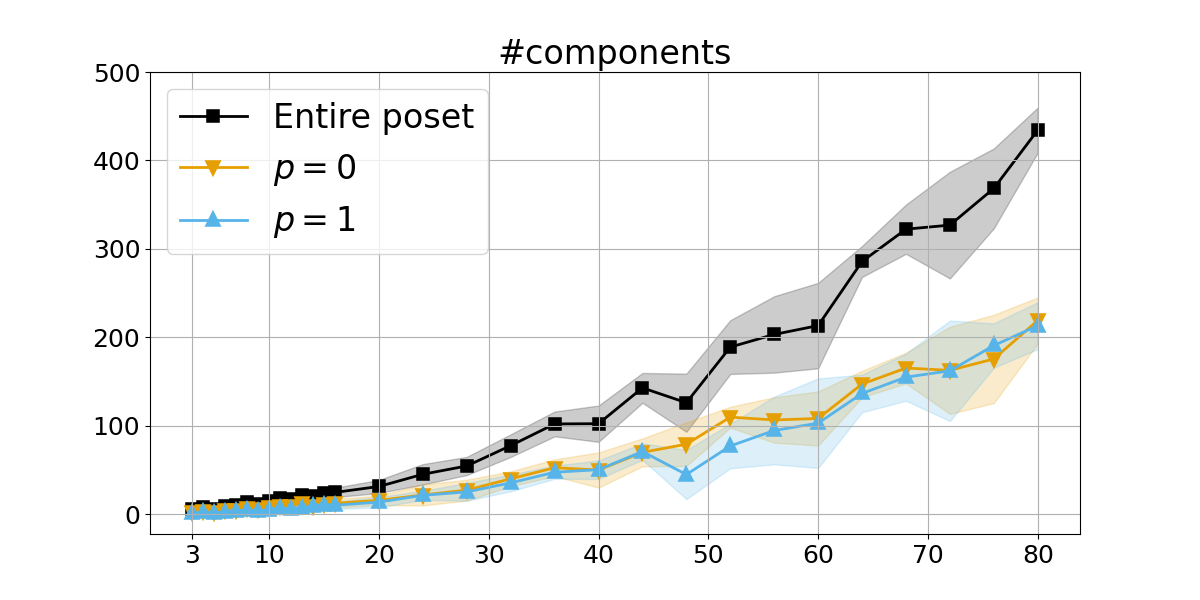
\includegraphics[width=1.4\textwidth]{pics/extended torus scores/score=number-of-components, dim=2, object=full.png}
        \caption{Score number\_of\_components values for the full poset of $\mathbb{T}_n^{2}$.}
        \label{fig:numberofcomponents-full2}
    \end{figure}
    \begin{figure}[h!]
        \centering
        \hspace*{-0.24\textwidth}
        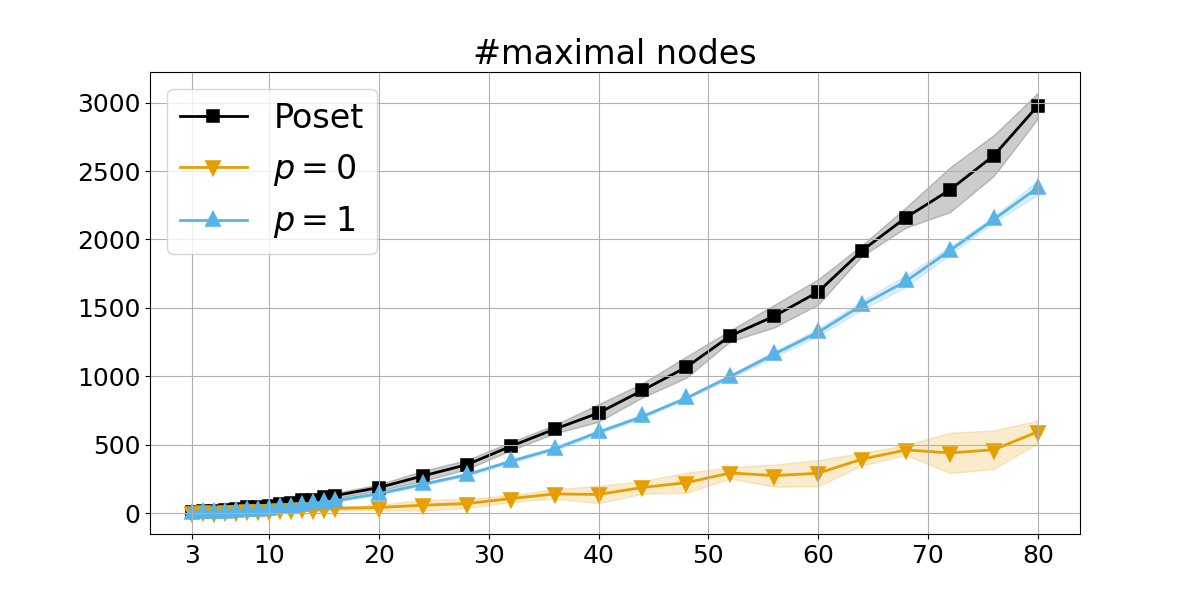
\includegraphics[width=1.4\textwidth]{pics/extended torus scores/score=number-of-maximal-nodes, dim=2, object=row reduction.png}
        \caption{Score number\_of\_maximal\_nodes values for the row reduction poset of $\mathbb{T}_n^{2}$.}
        \label{fig:numberofmaximalnodes-rowreduction2}
    \end{figure}
    \begin{figure}[h!]
        \centering
        \hspace*{-0.24\textwidth}
        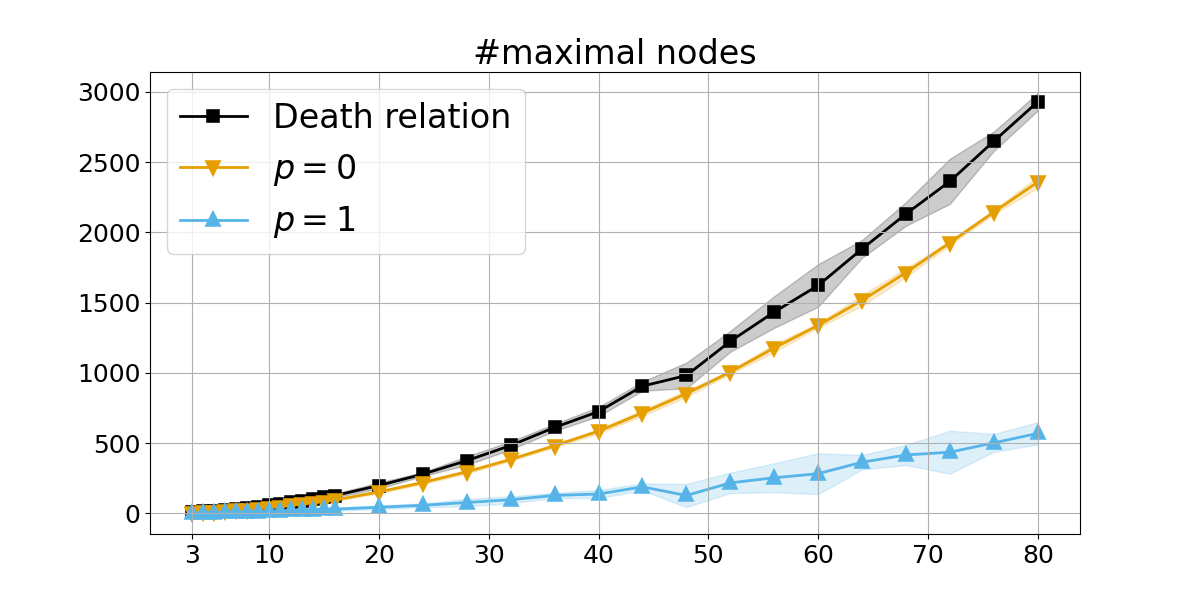
\includegraphics[width=1.4\textwidth]{pics/extended torus scores/score=number-of-maximal-nodes, dim=2, object=column reduction.png}
        \caption{Score number\_of\_maximal\_nodes values for the column reduction poset of $\mathbb{T}_n^{2}$.}
        \label{fig:numberofmaximalnodes-columnreduction2}
    \end{figure}
    \begin{figure}[h!]
        \centering
        \hspace*{-0.24\textwidth}
        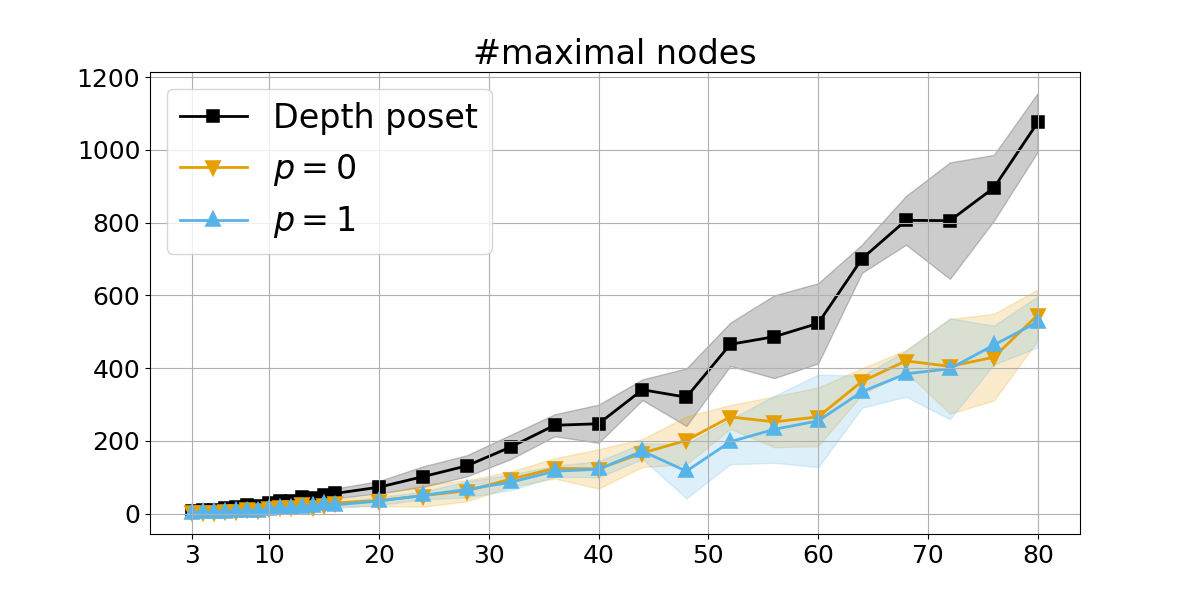
\includegraphics[width=1.4\textwidth]{pics/extended torus scores/score=number-of-maximal-nodes, dim=2, object=full.png}
        \caption{Score number\_of\_maximal\_nodes values for the full poset of $\mathbb{T}_n^{2}$.}
        \label{fig:numberofmaximalnodes-full2}
    \end{figure}
    \begin{figure}[h!]
        \centering
        \hspace*{-0.24\textwidth}
        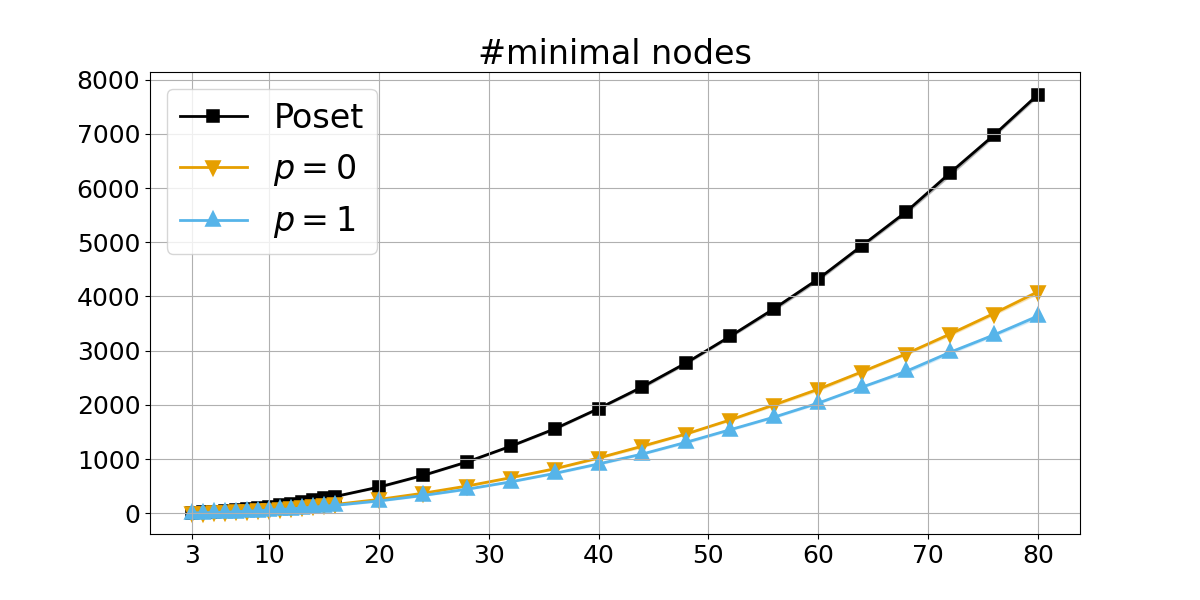
\includegraphics[width=1.4\textwidth]{pics/extended torus scores/score=number-of-minimal-nodes, dim=2, object=row reduction.png}
        \caption{Score number\_of\_minimal\_nodes values for the row reduction poset of $\mathbb{T}_n^{2}$.}
        \label{fig:numberofminimalnodes-rowreduction2}
    \end{figure}
    \begin{figure}[h!]
        \centering
        \hspace*{-0.24\textwidth}
        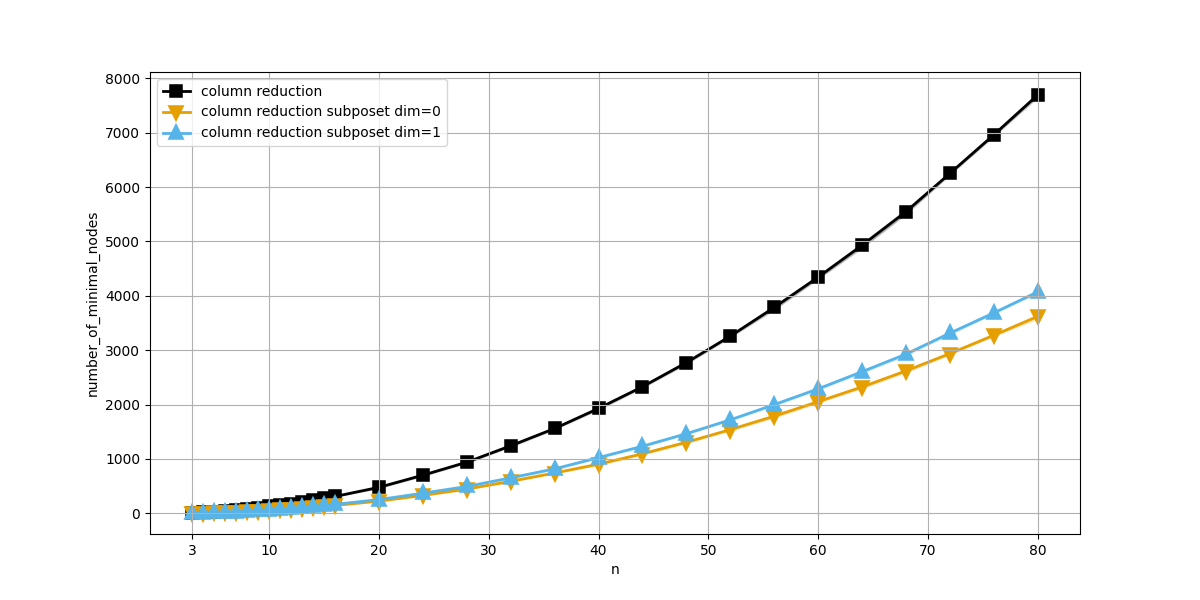
\includegraphics[width=1.4\textwidth]{pics/extended torus scores/score=number-of-minimal-nodes, dim=2, object=column reduction.png}
        \caption{Score number\_of\_minimal\_nodes values for the column reduction poset of $\mathbb{T}_n^{2}$.}
        \label{fig:numberofminimalnodes-columnreduction2}
    \end{figure}
    \begin{figure}[h!]
        \centering
        \hspace*{-0.24\textwidth}
        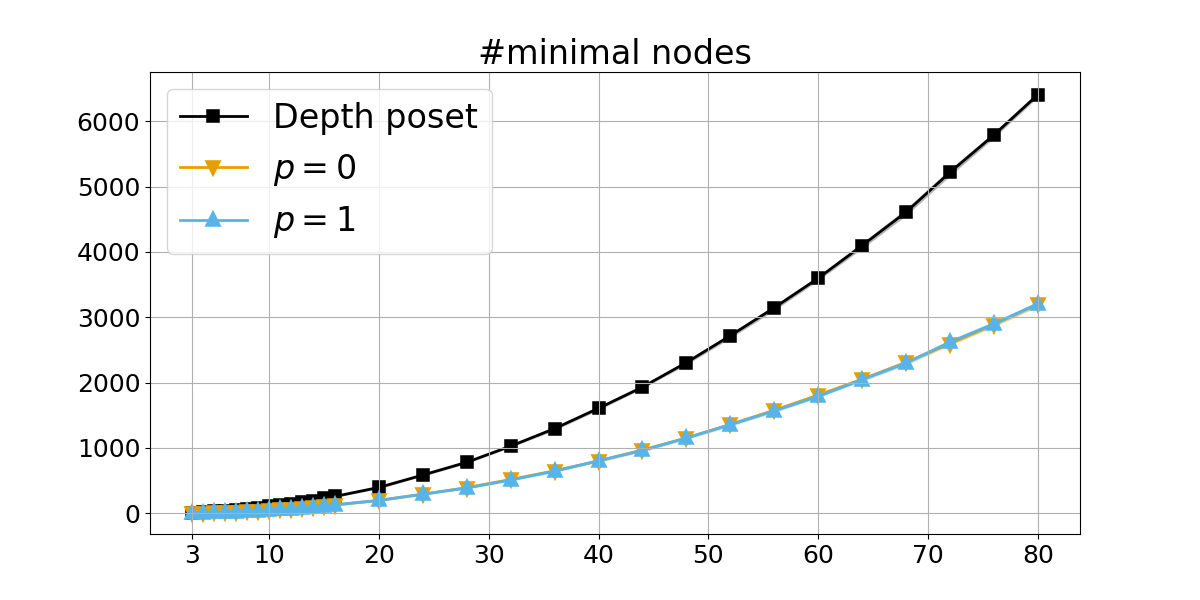
\includegraphics[width=1.4\textwidth]{pics/extended torus scores/score=number-of-minimal-nodes, dim=2, object=full.png}
        \caption{Score number\_of\_minimal\_nodes values for the full poset of $\mathbb{T}_n^{2}$.}
        \label{fig:numberofminimalnodes-full2}
    \end{figure}
    \begin{figure}[h!]
        \centering
        \hspace*{-0.24\textwidth}
        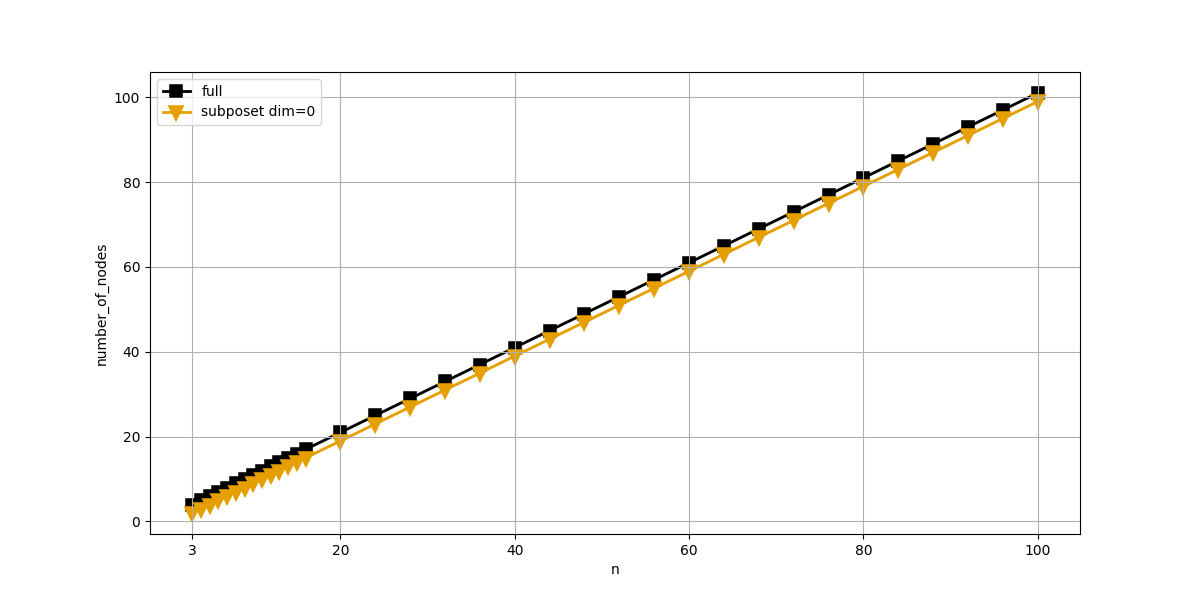
\includegraphics[width=1.4\textwidth]{pics/extended torus scores/score=number-of-nodes, dim=1, object=full.png}
        \caption{Score number\_of\_nodes values for the full poset of $\mathbb{T}_n^{1}$.}
        \label{fig:numberofnodes-full1}
    \end{figure}
    \begin{figure}[h!]
        \centering
        \hspace*{-0.24\textwidth}
        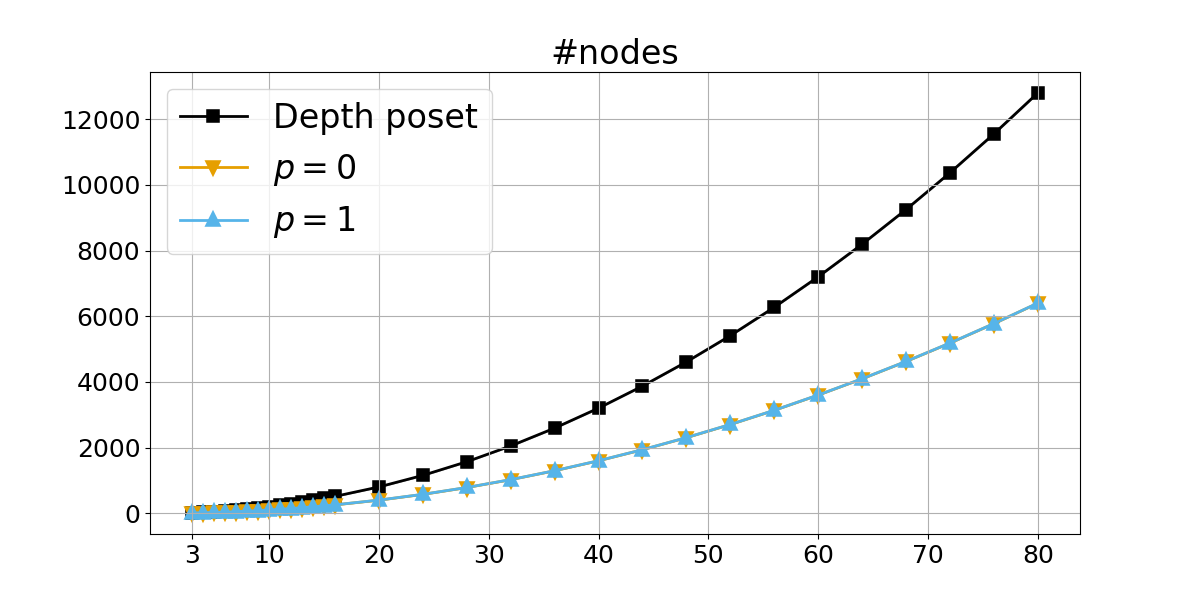
\includegraphics[width=1.4\textwidth]{pics/extended torus scores/score=number-of-nodes, dim=2, object=full.png}
        \caption{Score number\_of\_nodes values for the full poset of $\mathbb{T}_n^{2}$.}
        \label{fig:numberofnodes-full2}
    \end{figure}
    \begin{figure}[h!]
        \centering
        \hspace*{-0.24\textwidth}
        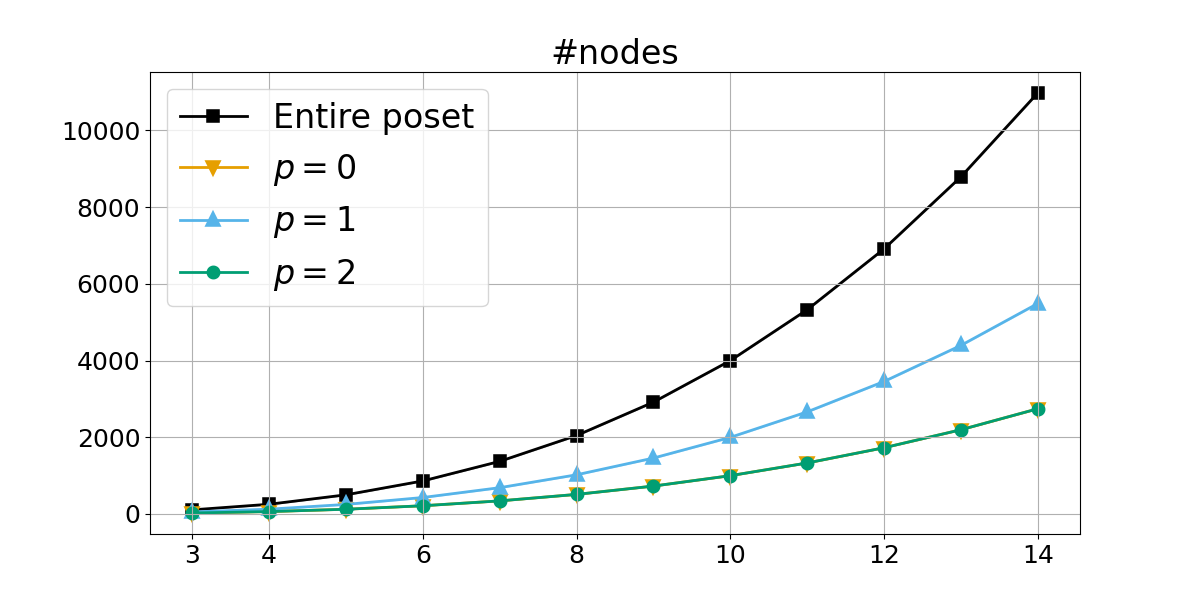
\includegraphics[width=1.4\textwidth]{pics/extended torus scores/score=number-of-nodes, dim=3, object=full.png}
        \caption{Score number\_of\_nodes values for the full poset of $\mathbb{T}_n^{3}$.}
        \label{fig:numberofnodes-full3}
    \end{figure}
    \begin{figure}[h!]
        \centering
        \hspace*{-0.24\textwidth}
        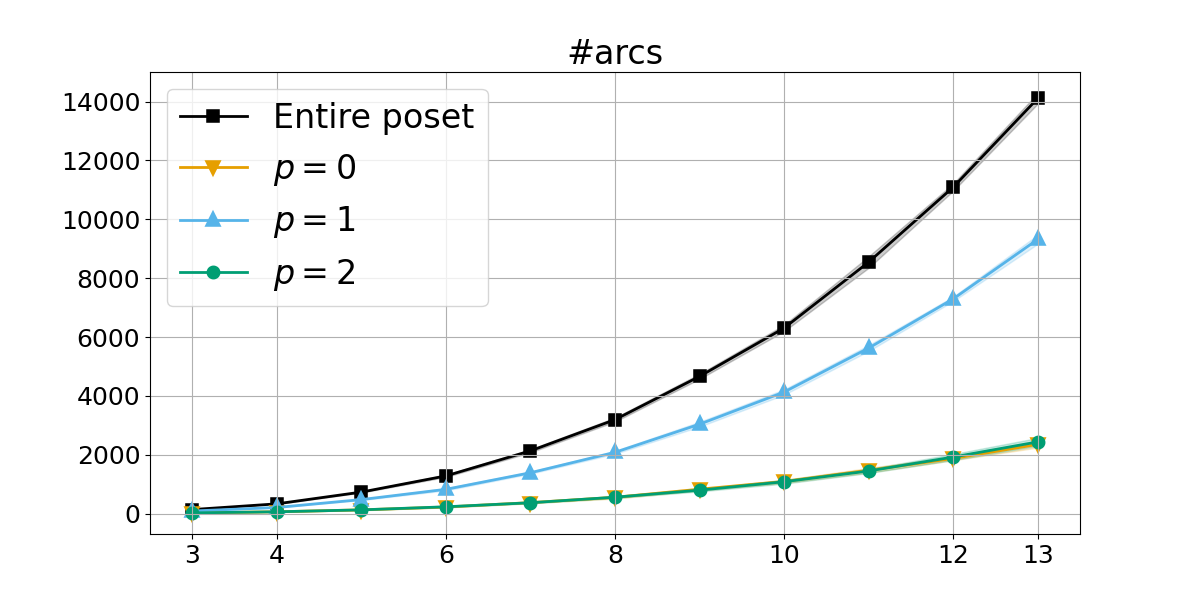
\includegraphics[width=1.4\textwidth]{pics/extended torus scores/score=number-of-relations, dim=3, object=full.png}
        \caption{Score number\_of\_relations values for the full poset of $\mathbb{T}_n^{3}$.}
        \label{fig:numberofrelations-full3}
    \end{figure}
    \begin{figure}[h!]
        \centering
        \hspace*{-0.24\textwidth}
        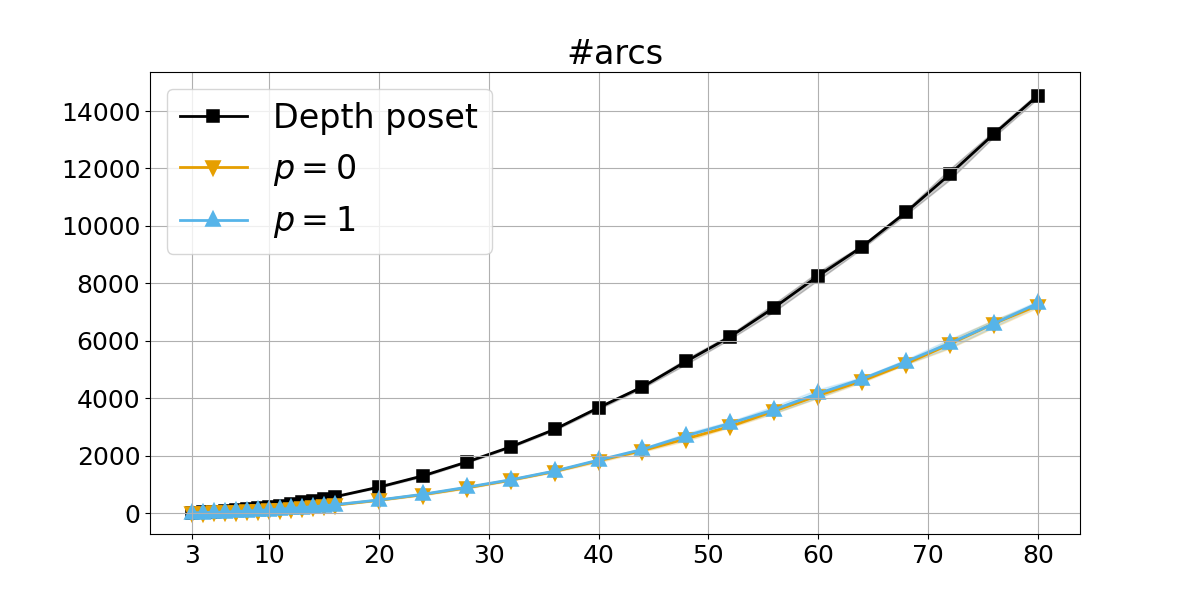
\includegraphics[width=1.4\textwidth]{pics/extended torus scores/score=number-of-relations, dim=2, object=full.png}
        \caption{Score number\_of\_relations values for the full poset of $\mathbb{T}_n^{2}$.}
        \label{fig:numberofrelations-full2}
    \end{figure}
    \begin{figure}[h!]
        \centering
        \hspace*{-0.24\textwidth}
        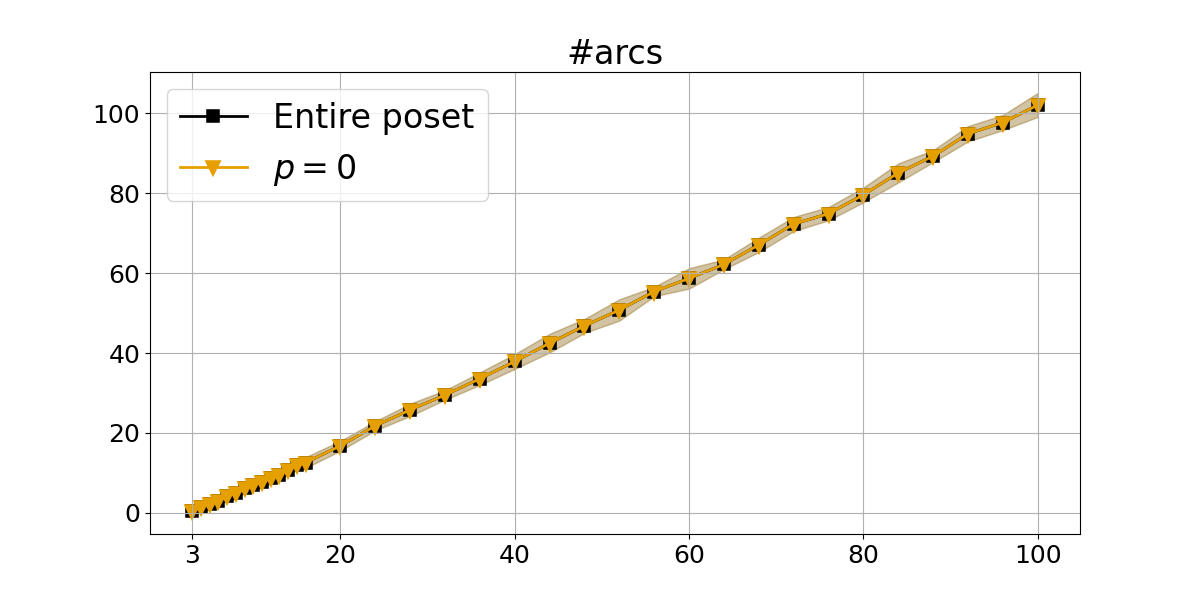
\includegraphics[width=1.4\textwidth]{pics/extended torus scores/score=number-of-relations, dim=1, object=full.png}
        \caption{Score number\_of\_relations values for the full poset of $\mathbb{T}_n^{1}$.}
        \label{fig:numberofrelations-full1}
    \end{figure}


\end{document}